\chapter{CHI TIẾT CÁC THÀNH PHẦN CỐT LÕI}

\section{Backend (Node.js \& Express)}
\subsection{Vai trò và Nhiệm vụ}
\subsection{Tech Stack \& Thư viện}
\subsection{Quy trình xử lý}

\section{Frontend (Flutter Multi-platform)}

\subsection{Vai trò và Nhiệm vụ}

\quad Frontend đóng vai trò lớp giao tiếp trực tiếp giữa người dùng và hệ thống TourXport, chịu trách nhiệm xây dựng giao diện, xử lý tương tác và hiển thị dữ liệu một cách trực quan.

\quad Trong dự án TourXport, frontend được phát triển bằng Flutter \cite{fe1} nhằm hỗ trợ đa nền tảng và đảm bảo tính đồng nhất về giao diện trên các thiết bị di động.

\quad Nhiệm vụ chính của frontend trong giai đoạn POC:

\begin{itemize}
    \item Xây dựng Trải nghiệm Người dùng (UX)
    \item Phát triển Giao diện (UI) \cite{fe2}
    \item Thu thập Dữ liệu Người dùng
    \item Xử lý và Hiển thị Dữ liệu
    \item Quản lý Tài khoản
\end{itemize}

\subsection{Tech Stack \& Thư viện}

\quad Front-end của TourXport được xây dựng trên nền tảng công nghệ hiện đại nhằm đảm bảo hiệu năng và tính thẩm mỹ cao:

\begin{itemize}
    \item \textbf{Framework chính}: Flutter cho phép xây dựng ứng dụng đa nền tảng (Android, iOS, Web, Windows) từ một codebase duy nhất.
    \item \textbf{Ngôn ngữ lập trình}: Dart \cite{fe3} là ngôn ngữ tối ưu cho việc xây dựng UI và các tác vụ bất đồng bộ.
    \item \textbf{Thư viện và Công cụ} \cite{fe5}:
        \begin{itemize}
            \item http: Xử lý các yêu cầu mạng (RESTful API) tới Backend.
            \item google\_fonts: Tích hợp bộ font chữ Montserrat chuyên nghiệp
        \end{itemize}
    \item \textbf{Công cụ hỗ trợ}: Figma - thiết kế UI/UX và prototype giao diện
\end{itemize}

\subsection{Quy trình xử lý}

\quad \textbf{Bước 1}: Lên ý tưởng và phân tích yêu cầu
\begin{itemize}
    \item Xác định chức năng cần phát triển
    \item Phân tích nhu cầu người dùng
    \item Xây dựng luồng sử dụng của ứng dụng
\end{itemize}

\quad \textbf{Bước 2}: Thiết kế giao diện trên Figma \cite{fe4}
\begin{itemize}
    \item Chọn màu sắc, font chữ, bố cục
    \item Tạo prototype mô phỏng trải nghiệm người dùng
\end{itemize}

\quad \textbf{Bước 3}: Phát triển giao diện bằng Dart với Flutter
\begin{itemize}
    \item Chuyển thiết kế thành giao diện thực tế
    \item Xây dựng widget và xử lý logic frontend
    \item Kết nối API và quản lý trạng thái ứng dụng
\end{itemize}

\quad \textbf{Bước 4}: Kiểm thử trên máy ảo
\begin{itemize}
    \item Chạy thử trên Android Emulator
    \item Kiểm tra responsive và hiệu năng
    \item Phát hiện và sửa lỗi giao diện/chức năng
\end{itemize}

\subsection{Phân chia công việc}

\subsubsection{Sprint 1}

\begin{figure}[H]
    \centering
    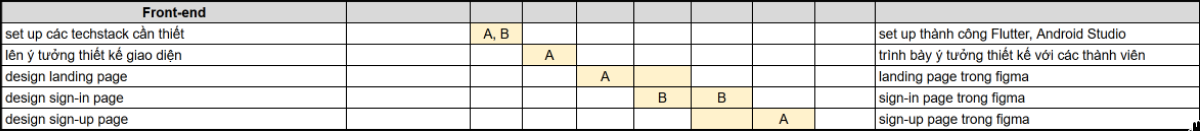
\includegraphics[width=1\textwidth]{img/FEsprint1-1.png}
    \caption{Bảng theo dõi công việc front-end sprint 1}
\end{figure}

\quad Trong Sprint 1, nhóm Front-end tập trung xây dựng nền tảng ban đầu cho ứng dụng bằng Flutter và ngôn ngữ Dart. Mục tiêu chính của sprint là hoàn thành môi trường phát triển, lên ý tưởng giao diện và thiết kế các màn hình cơ bản trên Figma để chuẩn bị cho giai đoạn lập trình.

\quad Các công việc đã thực hiện gồm:
\begin{itemize}
    \item Cài đặt và cấu hình các công nghệ cần thiết như Flutter, Dart và Android Studio.
    \item Thảo luận và thống nhất ý tưởng thiết kế giao diện với các thành viên trong nhóm.
    \item Thiết kế landing page, sign-in page và sign-up page trên Figma.
    \item Xây dựng cấu trúc dự án Flutter ban đầu và kiểm tra khả năng chạy ứng dụng trên máy ảo Android Emulator.
\end{itemize}

\begin{figure}[H]
    \centering
    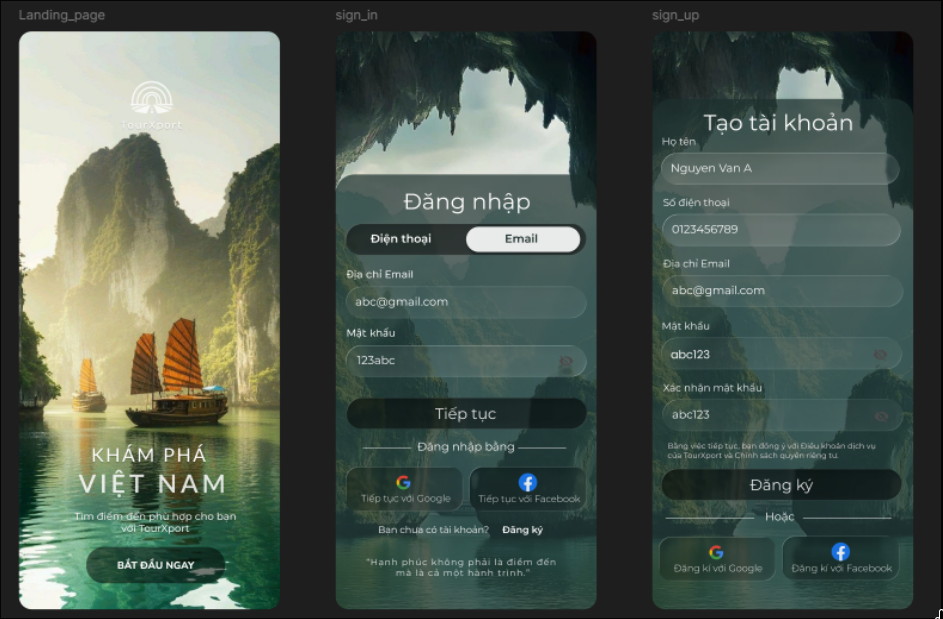
\includegraphics[width=1\textwidth]{img/FEsprint1-2.png}
    \caption{Thiết kế landing page, sign in, sign up}
\end{figure}

\quad Kết quả đạt được sau Sprint 1:
\begin{itemize}
    \item Môi trường phát triển Front-end đã được thiết lập hoàn chỉnh.
    \item Bộ giao diện cơ bản đã được thiết kế thống nhất.
    \item Ứng dụng Flutter có thể khởi chạy và chạy thử nghiệm thành công trên máy ảo.
\end{itemize}

\subsubsection{Sprint 2}

\begin{figure}[H]
    \centering
    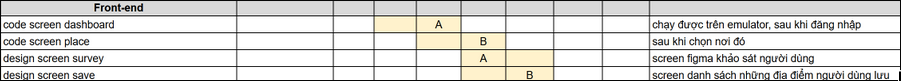
\includegraphics[width=0.9\textwidth]{img/FEsprint2-1.png}
    \caption{Bảng theo dõi công việc front-end sprint 2}
\end{figure}

\quad Trong Sprint 2, nhóm tiếp tục phát triển các chức năng chính của ứng dụng bằng Flutter và Dart. Sprint này tập trung vào việc xây dựng các màn hình chức năng sau khi người dùng đăng nhập, đồng thời mở rộng thiết kế giao diện phục vụ trải nghiệm cá nhân hóa.

\quad Các công việc đã thực hiện gồm:
\begin{itemize}
    \item Phát triển màn hình Dashboard và tích hợp điều hướng cơ bản sau khi đăng nhập.
    \item Xây dựng màn hình Place để hiển thị danh sách địa điểm và chức năng chọn nơi đến.
    \item Thiết kế màn hình Survey nhằm khảo sát sở thích và nhu cầu của người dùng.
    \item Thiết kế màn hình Save để hiển thị danh sách các địa điểm đã được lưu.
\end{itemize}

\begin{figure}[H]
    \centering
    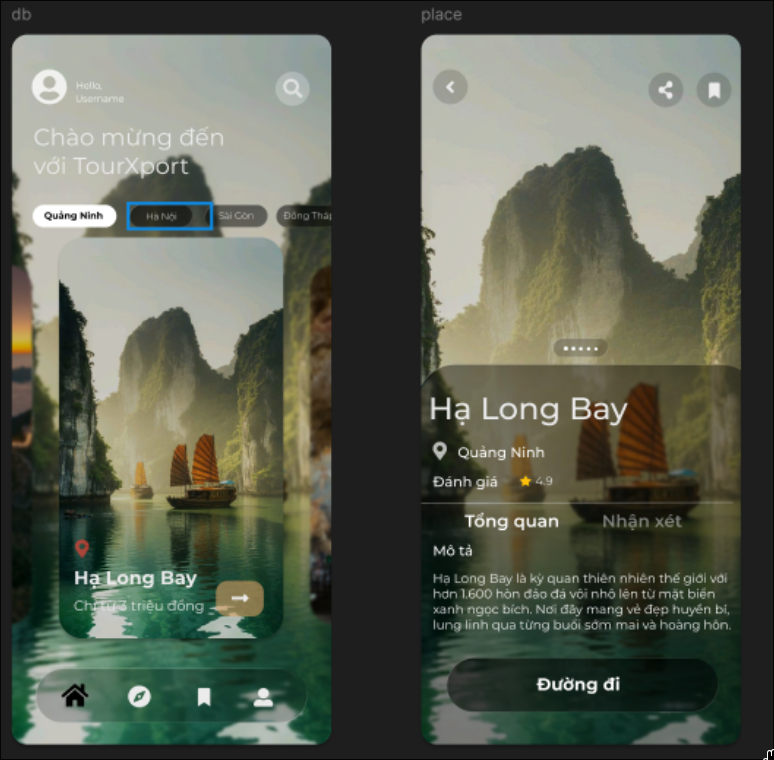
\includegraphics[width=0.6\textwidth]{img/FEsprint2-2.png}
    \caption{Thiết kế dashboard và places}
\end{figure}

\quad Kết quả đạt được sau Sprint 2:
\begin{itemize}
    \item Ứng dụng có thể điều hướng giữa các màn hình chính trên Android Emulator.
    \item Các chức năng giao diện cơ bản sau đăng nhập đã được xây dựng thành công.
    \item Hệ thống giao diện tiếp tục được hoàn thiện và đồng bộ theo thiết kế trên Figma.
\end{itemize}

\subsubsection{Sprint 3}

\begin{figure}[H]
    \centering
    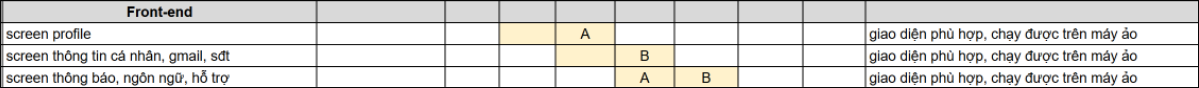
\includegraphics[width=1\textwidth]{img/FEsprint3-1.png}
    \caption{Bảng theo dõi công việc front-end sprint 3}
\end{figure}

\quad Trong Sprint 3, tiếp tục hoàn thiện các chức năng liên quan đến tài khoản và trải nghiệm người dùng bằng Flutter và Dart. Sprint này tập trung phát triển các màn hình cá nhân hóa và cài đặt trong ứng dụng.

\quad Các công việc đã thực hiện gồm:
\begin{itemize}
    \item Xây dựng màn hình Profile với giao diện phù hợp và khả năng hoạt động trên máy ảo.
    \item Phát triển màn hình thông tin cá nhân bao gồm họ tên, Gmail và số điện thoại.
    \item Thiết kế và hoàn thiện màn hình Thông báo, Ngôn ngữ và Hỗ trợ.
    \item Tối ưu bố cục giao diện nhằm đảm bảo tính đồng bộ và thân thiện với người dùng.
\end{itemize}

\begin{figure}[H]
    \centering
    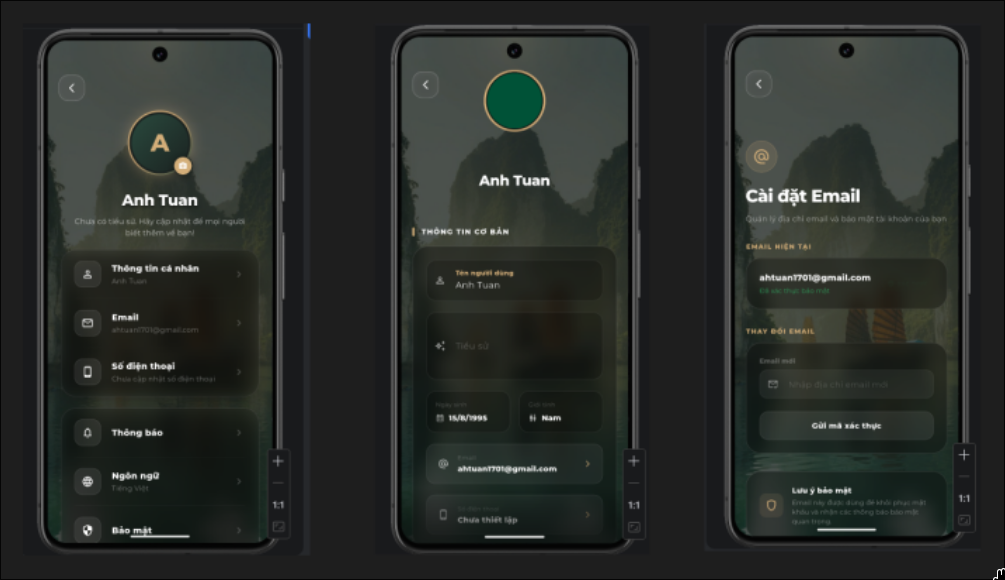
\includegraphics[width=0.9\textwidth]{img/FEsprint3-2.png}
    \caption{Màn hình máy ảo profile và trang thông tin cá nhân, email}
\end{figure}

\quad Kết quả đạt được sau Sprint 3:
\begin{itemize}
    \item Các màn hình quản lý tài khoản và cài đặt đã được xây dựng thành công.
    \item Ứng dụng tiếp tục hoạt động ổn định trên Android Emulator.
    \item Giao diện người dùng được hoàn thiện hơn về tính trực quan và trải nghiệm sử dụng.
\end{itemize}

\section{AI Worker (LLM \& RAG Engine)}
\subsection{Vai trò và Nhiệm vụ}
\subsection{Tech Stack \& Thư viện}
\subsection{Quy trình xử lý}

\section{Thu thập Dataset (Data Crawler/Scraper)}
\subsection{Vai trò và Nhiệm vụ}
\subsection{Tech Stack \& Thư viện}
\subsection{Quy trình xử lý}
